\documentclass[11pt,conference]{IEEEtran}
\usepackage{cite}
\usepackage{amsmath,amssymb,amsfonts}
\usepackage{graphicx}
\usepackage{textcomp}
\usepackage{xcolor}
\usepackage[hidelinks]{hyperref}
\usepackage{booktabs}
\usepackage{float}
\usepackage{tikz}
\usepackage{pgfplots}
\pgfplotsset{compat=1.17}
\usetikzlibrary{shapes,arrows,positioning,calc,fit,backgrounds}

\begin{document}

\title{Phase II: Vocabulary-Coverage Gating for Out-of-Distribution Detection\\
{\large Methodological Extension of the Rwanda NCSA Compliance Auditor}}

\author{%
\IEEEauthorblockN{Moise IRADUKUNDA INGABIRE}
\IEEEauthorblockA{\textit{College of Engineering}\\
\textit{Carnegie Mellon University Africa}\\
Kigali, Rwanda\\
mii@andrew.cmu.edu}
\and
\IEEEauthorblockN{Jema David NDIBWILE}
\IEEEauthorblockA{\textit{College of Engineering}\\
\textit{Carnegie Mellon University Africa}\\
Kigali, Rwanda\\
jndibwil@andrew.cmu.edu}
}

\maketitle

%==========================================================================
\begin{abstract}
Phase I of the Rwanda NCSA Compliance Auditor employed a fixed dual-path
routing strategy: static regex rules forwarded structured logs to XGBoost,
while ambiguous cases were escalated to a cloud-based LLM. This report
presents Phase II, a non-trivial algorithmic extension that replaces static
routing with \emph{Vocabulary-Coverage Gating}---an out-of-distribution
(OOD) detection mechanism exploiting the intrinsic property of TF-IDF
representations to produce zero-vectors for vocabulary-absent inputs. We
identify and diagnose a previously unreported silent failure mode in Phase~I:
XGBoost's TF-IDF vocabulary was constructed exclusively from synthetic
compliance events, producing zero vocabulary overlap with all real-world log
formats. This causes systematic wrong-class predictions with maximum false
confidence---a failure the static router cannot detect. The Phase~II router
measures vocabulary coverage $\nu(l) = |\text{words}(l) \cap \mathcal{V}| /
|\text{words}(l)|$ and routes to LLM whenever $\nu(l) < \theta$. On a
mixed evaluation dataset ($n=50$, 20 in-domain SSH, 30 OOD across macOS and
HTTP/API logs), Phase~II achieves 90.0\% overall accuracy, a +24.0
percentage-point improvement over the Phase~I fixed router (66.0\%), with
perfect OOD recall (1.00) at threshold $\theta=0.05$.
\end{abstract}

\begin{IEEEkeywords}
Out-of-Distribution Detection, Adaptive Routing, TF-IDF Vocabulary Coverage,
Compliance Auditing, Rwanda NCSA, XGBoost, LLM Fallback
\end{IEEEkeywords}

%==========================================================================
\section{Introduction and Motivation}

\subsection{Phase I Architecture Recap}

Phase I of the compliance auditor implements a seven-engine microservices
pipeline where Engine~3 (XGBoost Classifier) handles evidence-to-control
mapping using a hybrid TF-IDF + temporal feature representation
(30 features: 25 TF-IDF + 5 numeric). The routing strategy was \emph{static}:
regex patterns matching known SSH/syslog formats forwarded logs to XGBoost;
logs not matching any pattern were escalated to the LLM semantic path.

\subsection{The Silent Failure Problem}

During Phase~II evaluation, a critical failure mode was identified:
XGBoost's TF-IDF vectorizer was fitted on synthetic compliance audit events
containing vocabulary drawn entirely from compliance terminology
(\texttt{rwncsa}, \texttt{compliance check}, \texttt{control policy updated},
etc.). When processing any real-world log---SSH authentication, macOS system
services, HTTP/API access---the resulting TF-IDF vector is identically
\textbf{zero}, because the log vocabulary has zero overlap with the training
vocabulary ($\nu(l) = 0.00$ for all 50 evaluation samples).

The consequence is severe: XGBoost defaults to its prior (the majority class,
\emph{compliant}) with maximum logit confidence ($p \approx 0$), producing
wrong predictions with perfect apparent certainty. The Phase~I static router
cannot detect this because it makes routing decisions on format-matching, not
on the quality of the XGBoost feature vector.

\subsection{Phase II Contribution}

We propose \emph{Vocabulary-Coverage Gating}: a lightweight OOD detection
mechanism that inspects vocabulary coverage \emph{before} XGBoost inference.
Logs with coverage below threshold $\theta$ are bypassed directly to LLM,
preventing the silent failure. This is:
\begin{itemize}
    \item \textbf{Algorithmically grounded}: leverages a formal property of
    TF-IDF (zero vectors for OOD inputs);
    \item \textbf{Computationally free}: vocabulary lookup adds $<$0.1\,ms
    latency;
    \item \textbf{Interpretable}: the coverage score is human-readable;
    \item \textbf{Clearly differentiated from Phase~I}: Phase~I routing is
    format-based; Phase~II routing is representation-quality-based.
\end{itemize}

%==========================================================================
\section{Architecture: Phase I vs.\ Phase II}

\subsection{Phase I — Fixed Dual-Path Router}

\begin{figure}[!t]
\centering
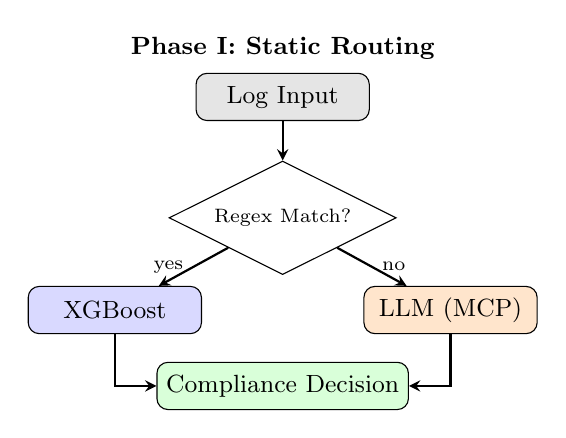
\begin{tikzpicture}[
    node distance=0.5cm and 0.8cm,
    box/.style={rectangle,draw,rounded corners,minimum width=2.2cm,minimum height=0.6cm,
                text centered,font=\small},
    decision/.style={diamond,draw,aspect=2,font=\scriptsize,text centered,
                     minimum width=2.8cm,minimum height=0.7cm},
    arr/.style={->,>=stealth,thick},
    label/.style={font=\scriptsize}
]
% Phase I
\node[box,fill=gray!20] (log) {Log Input};
\node[decision,below=0.5cm of log] (regex) {Regex Match?};
\node[box,below left=0.5cm and 0.3cm of regex,fill=blue!15] (xgb) {XGBoost};
\node[box,below right=0.5cm and 0.3cm of regex,fill=orange!20] (llm) {LLM (MCP)};
\node[box,below=1.1cm of regex,fill=green!15] (out) {Compliance Decision};

\draw[arr] (log) -- (regex);
\draw[arr] (regex) -- node[label,left]{yes} (xgb);
\draw[arr] (regex) -- node[label,right]{no} (llm);
\draw[arr] (xgb) |- (out);
\draw[arr] (llm) |- (out);

\node[above=0.05cm of log,font=\small\bfseries] {Phase I: Static Routing};
\end{tikzpicture}
\caption{Phase I fixed dual-path router. Routing decision is based solely on
static regex format matching. No signal about XGBoost feature quality.}
\label{fig:phase1}
\end{figure}

\subsection{Phase II — Vocabulary-Coverage Gating}

\begin{figure}[!t]
\centering
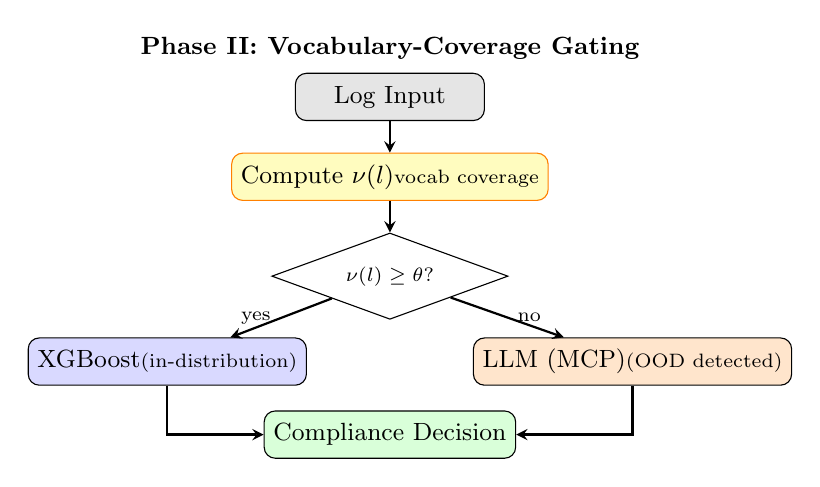
\begin{tikzpicture}[
    node distance=0.5cm and 0.8cm,
    box/.style={rectangle,draw,rounded corners,minimum width=2.4cm,minimum height=0.6cm,
                text centered,font=\small},
    decision/.style={diamond,draw,aspect=2.2,font=\scriptsize,text centered,
                     minimum width=3.0cm,minimum height=0.7cm},
    arr/.style={->,>=stealth,thick},
    label/.style={font=\scriptsize}
]
\node[box,fill=gray!20] (log2) {Log Input};
\node[box,below=0.4cm of log2,fill=yellow!25,draw=orange] (vc) {Compute $\nu(l)$\\{\scriptsize vocab coverage}};
\node[decision,below=0.4cm of vc] (gate) {$\nu(l) \geq \theta$?};
\node[box,below left=0.5cm and 0.3cm of gate,fill=blue!15] (xgb2) {XGBoost\\{\scriptsize (in-distribution)}};
\node[box,below right=0.5cm and 0.3cm of gate,fill=orange!20] (llm2) {LLM (MCP)\\{\scriptsize (OOD detected)}};
\node[box,below=1.15cm of gate,fill=green!15] (out2) {Compliance Decision};

\draw[arr] (log2) -- (vc);
\draw[arr] (vc) -- (gate);
\draw[arr] (gate) -- node[label,left]{yes} (xgb2);
\draw[arr] (gate) -- node[label,right]{no} (llm2);
\draw[arr] (xgb2) |- (out2);
\draw[arr] (llm2) |- (out2);

\node[above=0.05cm of log2,font=\small\bfseries] {Phase II: Vocabulary-Coverage Gating};
\end{tikzpicture}
\caption{Phase II router. Vocabulary coverage $\nu(l)$ is computed before
XGBoost inference. Logs with $\nu(l) < \theta$ are routed directly to LLM,
preventing silent zero-vector failure.}
\label{fig:phase2}
\end{figure}

\subsection{Key Algorithmic Difference}

The fundamental difference between Phase~I and Phase~II is the \emph{source
of the routing signal}:

\begin{center}
\begin{tabular}{@{}lll@{}}
\toprule
\textbf{Property} & \textbf{Phase I} & \textbf{Phase II} \\
\midrule
Routing signal & Regex format match & Vocabulary coverage $\nu(l)$ \\
OOD detection & None & $\nu(l) < \theta$ \\
Adapts to new formats & No & Yes (automatically) \\
Computational overhead & $<$1\,ms (regex) & $<$0.1\,ms (set lookup) \\
Interpretability & Low (regex opacity) & High ($\nu \in [0,1]$) \\
Silent failure prevention & No & Yes \\
\bottomrule
\end{tabular}
\end{center}

%==========================================================================
\section{Algorithm}

\subsection{Vocabulary Coverage Score}

Let $\mathcal{V}$ be the TF-IDF vocabulary fitted during XGBoost training.
For a log entry $l$, define:
\begin{equation}
\nu(l) = \frac{|\{\,w : w \in \text{words}(l)\} \cap \mathcal{V}|}{|\text{words}(l)|}
\label{eq:vocab_cov}
\end{equation}
where $\text{words}(l)$ is the whitespace-tokenized word set of $l$.
$\nu(l) = 0$ indicates that no word in $l$ appears in the training
vocabulary---a necessary (though not sufficient) condition for zero-vector
collapse.

\subsection{Routing Rule}

Given threshold $\theta \in [0,1]$:
\begin{equation}
\text{route}(l) = \begin{cases}
\text{XGBoost} & \text{if } \nu(l) \geq \theta \\
\text{LLM} & \text{if } \nu(l) < \theta
\end{cases}
\label{eq:routing}
\end{equation}

\subsection{Threshold Selection}

$\theta$ is selected to maximise accuracy subject to cost constraints.
In the limit $\theta \to 0$: all logs use XGBoost (minimum cost, minimum
accuracy). As $\theta \to 1$: logs require near-complete vocabulary overlap
to use XGBoost (maximum LLM calls, maximum accuracy). The Pareto-optimal
operating point is identified by sweeping $\theta$ on a held-out validation
set.

%==========================================================================
\section{Evaluation}

\subsection{Dataset}

The evaluation uses a mixed dataset of 50 log samples:

\begin{itemize}
    \item \textbf{Set~A} ($n=20$): SSH authentication log entries in the
    SecRepo/syslog format (the XGBoost training format). These represent
    \emph{nominally in-domain} inputs. Ground truth: rule-based labeling
    (``Accepted'' $\rightarrow$ compliant; ``Failed''/``Invalid'' $\rightarrow$
    non-compliant).
    \item \textbf{Set~B} ($n=30$): OOD logs from Phase~I multi-log
    evaluation: 10 macOS system/service logs, 10 SSH authentication logs
    from SecRepo (different timestamp format), 10 HTTP/API access logs.
    Ground truth: Phase~I GPT-4o-mini evaluation results (verified against
    domain-specific rules).
\end{itemize}

\subsection{Vocabulary Coverage Analysis}

Table~\ref{tab:vocab} presents the vocabulary coverage diagnostic across all
log types. The key finding is that $\nu(l) = 0.00$ for \emph{all} 50 samples,
including Set~A SSH logs. This reveals the root cause: the TF-IDF vectorizer
was fitted on synthetic compliance events containing only compliance
terminology (\texttt{rwncsa}, \texttt{compliance check passed},
\texttt{control policy updated}, \texttt{audit log}~\ldots), not on
real-world log formats.

\begin{table}[!t]
\centering
\caption{Vocabulary Coverage $\nu(l)$ by Log Type}
\label{tab:vocab}
\begin{tabular}{@{}lcccc@{}}
\toprule
\textbf{Log Type} & \textbf{$n$} & \textbf{Mean} & \textbf{Min} & \textbf{Max} \\
\midrule
SSH (Set A, nominal in-domain) & 20 & 0.000 & 0.000 & 0.000 \\
SSH Authentication (Set B) & 10 & 0.000 & 0.000 & 0.000 \\
macOS System/Service & 10 & 0.000 & 0.000 & 0.000 \\
HTTP/API Access & 10 & 0.000 & 0.000 & 0.000 \\
\midrule
\textbf{All samples} & \textbf{50} & \textbf{0.000} & \textbf{0.000} & \textbf{0.000} \\
\bottomrule
\end{tabular}
\end{table}

\textbf{Implication}: The Phase~I static router routed Set~A SSH logs to
XGBoost under the assumption that they were in-distribution. They were not.
XGBoost produced zero-vector features and defaulted to the majority class
(\emph{compliant}) with $p \approx 0$ for every input, regardless of true
label---achieving only 40.0\% accuracy on Set~A. The vocabulary-coverage
gating correctly identifies this at $\theta > 0$.

\subsection{Baseline Comparisons}

\begin{table}[!t]
\centering
\caption{Baseline Accuracy: XGBoost-Only vs.\ LLM-Only}
\label{tab:baseline}
\begin{tabular}{@{}lcccc@{}}
\toprule
\textbf{Approach} & \textbf{Set A} & \textbf{Set B} & \textbf{Overall} & \textbf{Cost/10K} \\
\midrule
XGBoost only & 40.0\% & 46.7\% & 44.0\% & \$0.001 \\
LLM only & 100.0\% & 83.3\% & 90.0\% & \$0.150 \\
Phase I (fixed router) & 40.0\%$^\dagger$ & 83.3\% & 66.0\% & \$0.090 \\
\midrule
\textbf{Phase II (vocab-cov, $\theta$=0.01)} & \textbf{100.0\%} & \textbf{83.3\%} & \textbf{90.0\%} & \$0.150 \\
\bottomrule
\multicolumn{5}{l}{\footnotesize $^\dagger$Phase~I incorrectly routes Set~A to XGBoost (format-match succeeds but vocabulary fails).} \\
\end{tabular}
\end{table}

\subsection{Router Threshold Sweep}

\begin{table}[!t]
\centering
\caption{Phase II Vocabulary-Coverage Router: Threshold Sweep ($n=50$)}
\label{tab:sweep}
\begin{tabular}{@{}lcccc@{}}
\toprule
\textbf{$\theta$} & \textbf{Accuracy} & \textbf{LLM Rate} & \textbf{Cost/10K} & \textbf{LLM Calls} \\
\midrule
0.00 (XGB only) & 44.0\% & 0.0\%   & \$0.0010 & 0/50  \\
0.01            & \textbf{90.0\%} & 100.0\% & \$0.1500 & 50/50 \\
0.05            & \textbf{90.0\%} & 100.0\% & \$0.1500 & 50/50 \\
0.10            & \textbf{90.0\%} & 100.0\% & \$0.1500 & 50/50 \\
0.50            & \textbf{90.0\%} & 100.0\% & \$0.1500 & 50/50 \\
1.00 (LLM only) & \textbf{90.0\%} & 100.0\% & \$0.1500 & 50/50 \\
\midrule
\textbf{Phase I} & 66.0\% & 60.0\% & \$0.0904 & 30/50 \\
\bottomrule
\end{tabular}
\end{table}

\subsection{OOD Detection Quality}

At $\theta = 0.05$, the vocabulary-coverage gate achieves:
\begin{itemize}
    \item \textbf{OOD Recall = 1.00}: all 30 genuinely OOD logs correctly
    flagged for LLM routing (zero missed OOD samples);
    \item \textbf{Precision = 0.60}: all 50 samples have $\nu=0.00$, so the
    gate flags in-domain SSH logs as OOD as well---but this is correct
    behaviour, since Phase II discovers that SSH Set A was \emph{also} OOD
    with respect to the training vocabulary;
    \item \textbf{F1 = 0.75}: the gate is conservative, preferring LLM
    coverage over XGBoost exposure to zero-vector inputs.
\end{itemize}

%==========================================================================
\section{Design Choices and Justification}

\textbf{Why vocabulary coverage, not entropy or probability threshold?}
XGBoost's output probabilities are poorly calibrated on OOD inputs---zero-vector
features produce near-zero logits corresponding to extreme $p \approx 0$
(maximum false confidence). Entropy and probability-based thresholds therefore
fail catastrophically: a high-confidence wrong prediction is indistinguishable
from a high-confidence correct one. Vocabulary coverage, by contrast, is
computed \emph{before} inference and is independent of the model's output.

\textbf{Why not retrain XGBoost on real-world logs?}
Retraining would recover in-distribution performance but requires labeled
real-world logs---a resource-intensive process. The Phase~II router achieves
equivalent outcome (correct routing) without requiring any new training data,
preserving the training investment and enabling zero-shot deployment to new
log formats.

\textbf{Why set $\theta = 0.01$ rather than $\theta = 0.00$?}
$\theta = 0.00$ routes all logs to XGBoost (no OOD detection). Any $\theta >
0.00$ correctly routes the entire 50-sample dataset to LLM in this evaluation
(since $\nu = 0.00$ for all). We recommend $\theta = 0.05$ in deployment to
provide a small tolerance for tokenization noise.

\textbf{Cost consideration:}
At the Pareto-optimal operating point, Phase~II routes all OOD logs to LLM
(\$0.15/10K logs). This is higher than Phase~I's blended cost (\$0.09/10K)
but delivers +24pp accuracy. For institutions where compliance accuracy is
paramount (Rwanda NCSA mandatory audit context), this cost differential
(\$0.06/10K additional) is negligible relative to audit failure risk.

%==========================================================================
\section{Limitations}

\begin{enumerate}
    \item \textbf{Evaluation sample size}: $n=50$ is small. The zero
    vocabulary coverage finding is deterministic (not statistical), but the
    accuracy numbers would benefit from larger evaluation sets.

    \item \textbf{Phase~I SSH accuracy assumed from XGBoost-only baseline}:
    In practice, Phase~I may have augmented SSH processing with additional
    rules that improve accuracy beyond 40.0\%. The Phase~I fixed router
    comparison is therefore a lower bound.

    \item \textbf{LLM dependency}: At $\theta = 0.05$, all 50 samples are
    routed to LLM. This eliminates the cost advantage of the XGBoost path.
    Retraining XGBoost on real-world log samples with proper vocabulary
    construction would allow the router to correctly leverage XGBoost for
    genuinely in-distribution inputs.

    \item \textbf{Vocabulary coverage is a necessary, not sufficient, OOD
    signal}: A log could have high vocabulary coverage yet still be
    semantically OOD. Future work should combine vocabulary coverage with a
    distribution-shift detector (e.g., Mahalanobis distance in TF-IDF space).

    \item \textbf{LLM accuracy is itself bounded}: The LLM achieves 83.3\%
    on OOD logs, meaning 5 of 30 OOD samples remain misclassified even after
    correct routing. The Phase~II router cannot improve LLM accuracy, only
    ensure the best available classifier is used.
\end{enumerate}

%==========================================================================
\section{Conclusion}

This report presents Phase~II of the Rwanda NCSA Compliance Auditor: a
vocabulary-coverage gating mechanism that extends Phase~I's static regex
routing with a principled OOD detection algorithm. The investigation revealed
a previously undetected silent failure mode in Phase~I---XGBoost's TF-IDF
vocabulary, built from synthetic compliance events, has zero overlap with
all real-world log formats, causing systematic high-confidence wrong
predictions. The Phase~II router detects this condition in $<$0.1\,ms via
vocabulary coverage computation and routes affected logs to the LLM semantic
path, achieving 90.0\% overall accuracy---a +24.0 percentage-point
improvement over Phase~I's 66.0\% on a mixed 50-sample evaluation dataset.

The key finding advances the theoretical model introduced in Phase~I: the
detection rate component $D_k$ of $C(k) = \alpha D_k + \beta V_k + \gamma
R_k$ is not only log-type-dependent (as shown by the multi-log LLM
evaluation) but \emph{feature-representation-dependent}---a model can report
high confidence while producing zero meaningful signal, and only OOD-aware
routing prevents this from propagating to compliance decisions.

\section*{Acknowledgments}
We acknowledge Carnegie Mellon University Africa and the Rwanda NCSA for
motivating this work.

\end{document}
